\documentclass{IOS-Book-Article}
\usepackage{mathptmx}
\usepackage{hyperref,url}
\usepackage{graphicx}
\usepackage{float}
\def\Eo{\mbox{\sc Ezo}}
\def\Ec{\mbox{\sc Ezo-CNN}}
\def\Ed{\mbox{\sc DeepEzo}}
\def\Mx{\mbox{\sc MoHex}}
\def\Mc{\mbox{\sc MoHex-CNN}}
\def\Mt{\mbox{\sc MoHex-3HNN}}
\def\Sol{\mbox{\sc Solver}}
\def\Fuego{\mbox{\sc Fuego}}

\def\hb{\hbox to 10.7 cm{}}

\begin{document}
\pagestyle{headings}
\def\thepage{}
\begin{frontmatter}              % The preamble begins here.
%\pretitle{Pretitle}
\title{MoHex3HNN defeats DeepEzo in Hex}
\markboth{}{2018 New Taipei City Computer Olympiad Report: to appear in ICGA Journal}
\author{\fnms{Chao} \snm{Gao}} and
\author{\fnms{Kei} \snm{Takada}} and
\author{\fnms{Ryan} \snm{Hayward}\thanks{Corresponding 
  author: hayward@ualberta.ca.}}

\runningauthor{AuthorA et al.}
\address{Department of Computing Science, University of Alberta, Canada}
\end{frontmatter}
\markboth{Gao, Takada, Hayward}{\Mt\ defeats \Ed\ in Hex 2018}

\begin{figure}[hbt]
\includegraphics[width=\columnwidth]{photos/awards.eps}\
\caption{From left, Kei Takada, Chao Gao, Ryan Hayward}
\end{figure}
%convert hex-medallists.jpg -gravity Center -crop 95x66%+0+0 -compress lzw eps2:a.eps

\section{The Tournaments}
There were two Hex tournaments at the 2018 Computer Olympiad in New Taipei City:
board-size 11$\times$11 and 
board-size 13$\times$13.\footnote{\cite{H17olyrptsource} has .sgf 
  game records and source files for this report.
  \cite{Hexgui} has an SGF (Smart Game Format) viewer.
  SGF was developed by \cite{SGF}.}
11$\times$11 is the original size proposed by Piet Hein, 
who invented Hex in 1942. 
All one-move openings on all $n$$\times$$n$ Hex boards up to 9$\times$9
have been solved by computers, as have two 10$\times$10 openings 
\cite{PawlH13}.
11$\times$11 positions with about 25 moves are often easily solved
by computers,
so in recent years a 13$\times$13 tournament has been added.

%13 J b2 a3 c12 (b11 a2 c2)
%11 J j2 b4(?) (c2 c10)

Due to visa problems, entries from China were unable to travel to Taiwan,
leaving two contestants for each tourament:
\Ed{} from Japan, 
by Kei Takada, supervised by Masahito Yamamoto;
and \Mt{} from Canada,
by Chao Gao, supervised by Ryan Hayward and Martin M\"{u}ller and
assisted by 
Jakub Pawlewicz,
Ashley Herman,
Joseph Meleshko,
Jiahao Li,
Paul Banse,
Siqi Yan,
Wai Yi Low
and
Xutong Zhao.
Gao and Pawlewicz developed a self-play game procedure,
and game statistics were then used to select opening moves.

\Mt\ is an AlphaGo-style neural net program that shares
much code from the earlier MoHex2.0 by 
Broderick Arneson, Philip Henderson, Aja Huang, 
Jakub Pawlewicz, Noah Weninger, Kenny Young and Ryan Hayward.
Some version of MoHex won the previous
eight Olympiad Hex competitions \cite{HW17}.
MoHex2.0 is an MCTS program that uses the Benzene Hex framework
built on the code base of \Fuego\ \cite{fuego}.

\Mt{}, the successor of \Mc,
uses a three-head convolutional neural net (CNN)
with 128 filters per layer \cite{ijcai}
and was trained on 400 000 self-play games.
At each new node of the Monte Carlo search tree, 
the three-headed neural net is called
and returns policy, state, and action values.
\Mt{} ran remotely on a machine with four CPU cores and one GPU.
For this tournament, all threads were used for tree computation,
rather than reserving one or more threads for a solver.

%\Eo{}, based on the Benzene framework, 
%uses iterative deepening alpha-beta search 
%with policy and value functions
%learned from 10 000 000 self-play games
%generated by minimax search.
\Ed{} ran remotely on a machine
with two CPUs and one GPU.
In some games the internet connection was dropped
and computation restarted on a  laptop.
with one CPU-thread for search and one CPU-thread for
Benzene's Depth-First Proof Number Search endgame solver.

\Ed{}, based on the Benzene framework,
uses iterative deepening depth-first search and 
two CNN functions.
One is the evaluation function, which evaluates the current position.
The other is the policy function, 
which decides which moves to search next.
Moves whose value exceed a threshold are explored;
the rest are pruned.

These two functions are created using reinforcement learning.
The functions are initialized to random weights.
The games used for learning are generated by self-play using
depth-one minimax search.

On a 13$\times$13 board,
\Ed{} won about .80 and .85 of its games respectively against
MoHex2.0 and \Ec{}(2017).
\Ed{} and MoHex2.0 were allowed 30s/move, and \Ec{}(2017) 
was allowed 4-ply search.
676 games were used for testing:
two games each as first player and then second player, over all opening moves.

The \Ed{} model used in this competition had more
learning than the tested movdel, so might be even stronger.
In the learning process, 2.6 million games have been played so far.

{\bf Tournament results.}
Each tournament was best of 8 games,
with 30min/game per player.
The 13$\times$13 and 11$\times$11 tournaments were played
on July 8 and 9 respectively.
Each game ended by resignation as soon as an opponent win was detected.
\Mt\ won both tournaments 5-0.

\section{13$\times$13 Games}
In a game, if the second move is `swap', then players
exchange colors and the first player plays the next move:
in the corresponding diagram, black `S' marks the first two moves
and white `3' the next move.
In the figures, `X-Y 1-0' indicates that X plays first, starting as black, 
and X wins (as white if B swapped, as black if not).

\begin{figure}
\noindent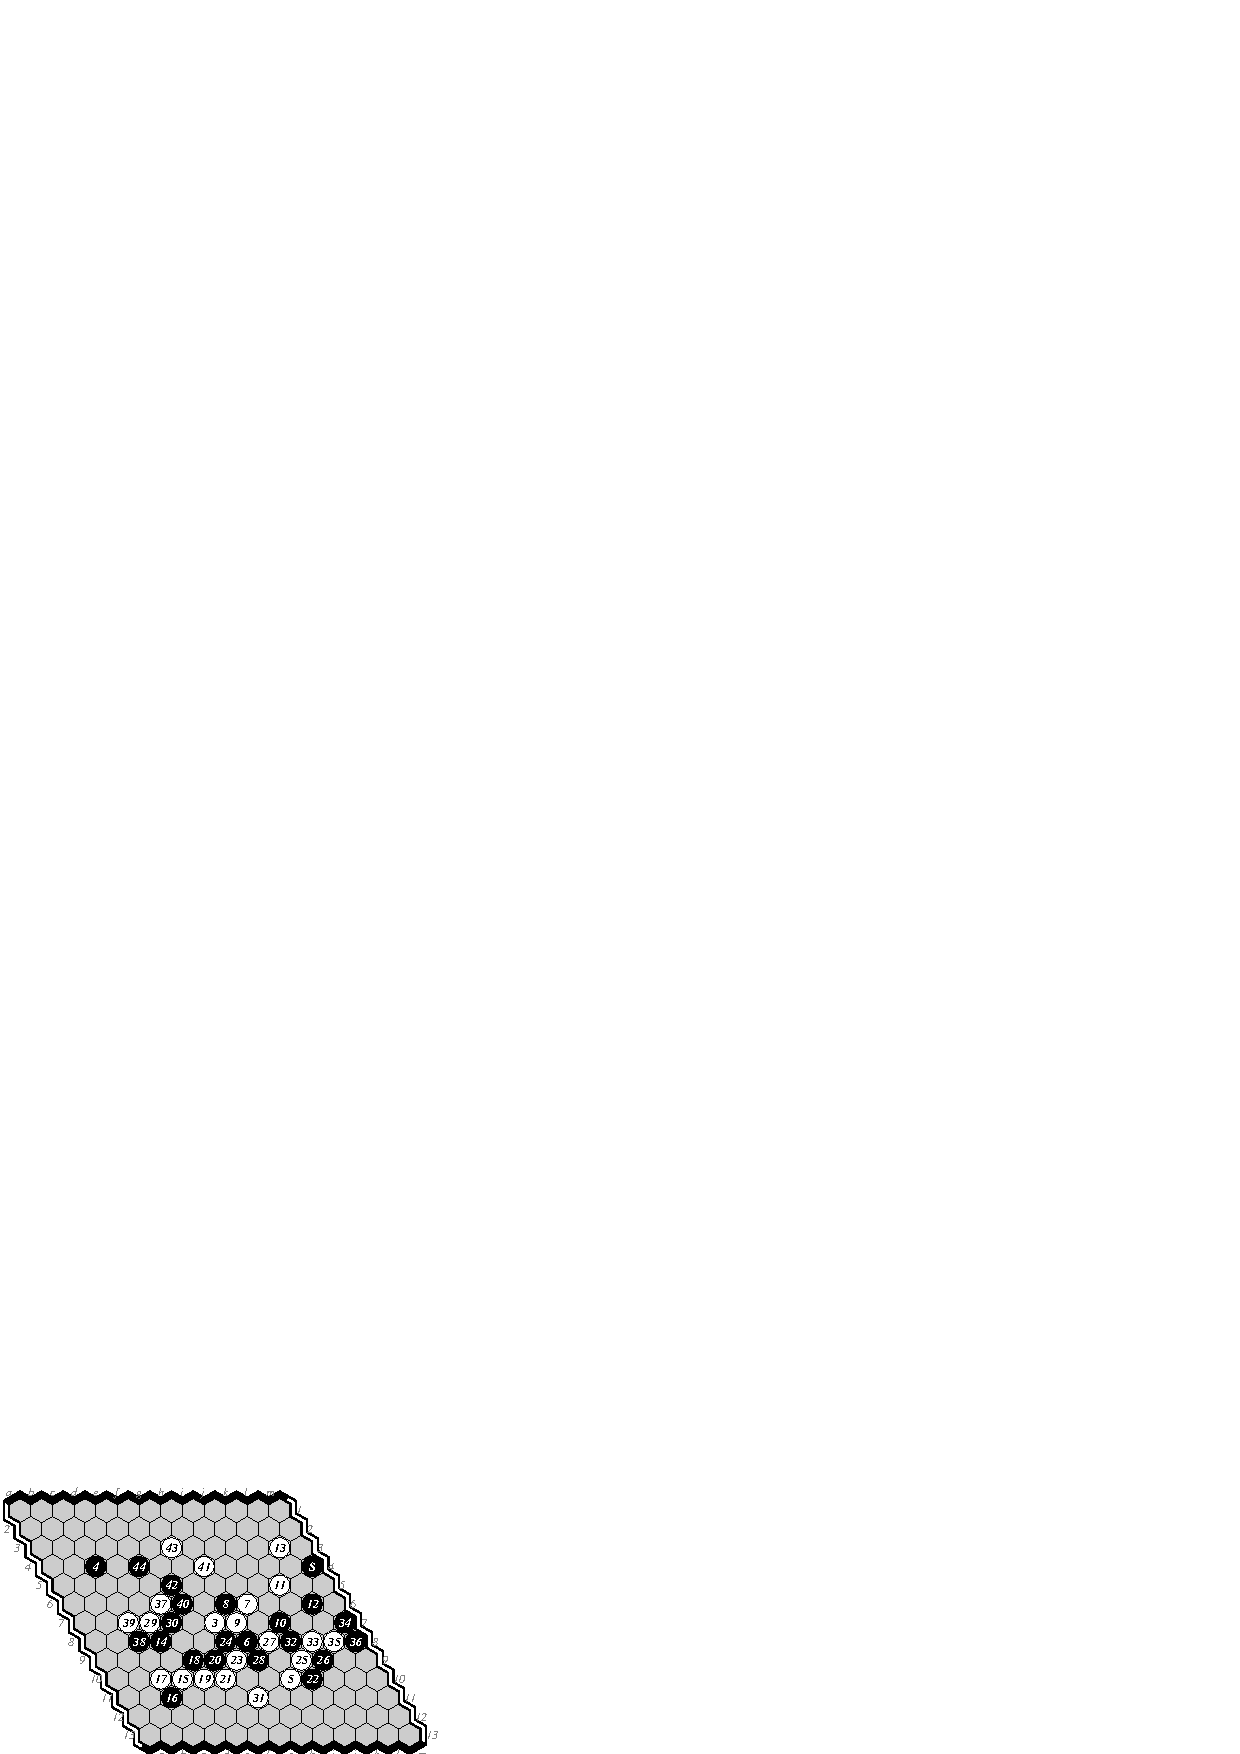
\includegraphics[width=.58\columnwidth]{pix/01-e-m}\hspace*{-.14\columnwidth}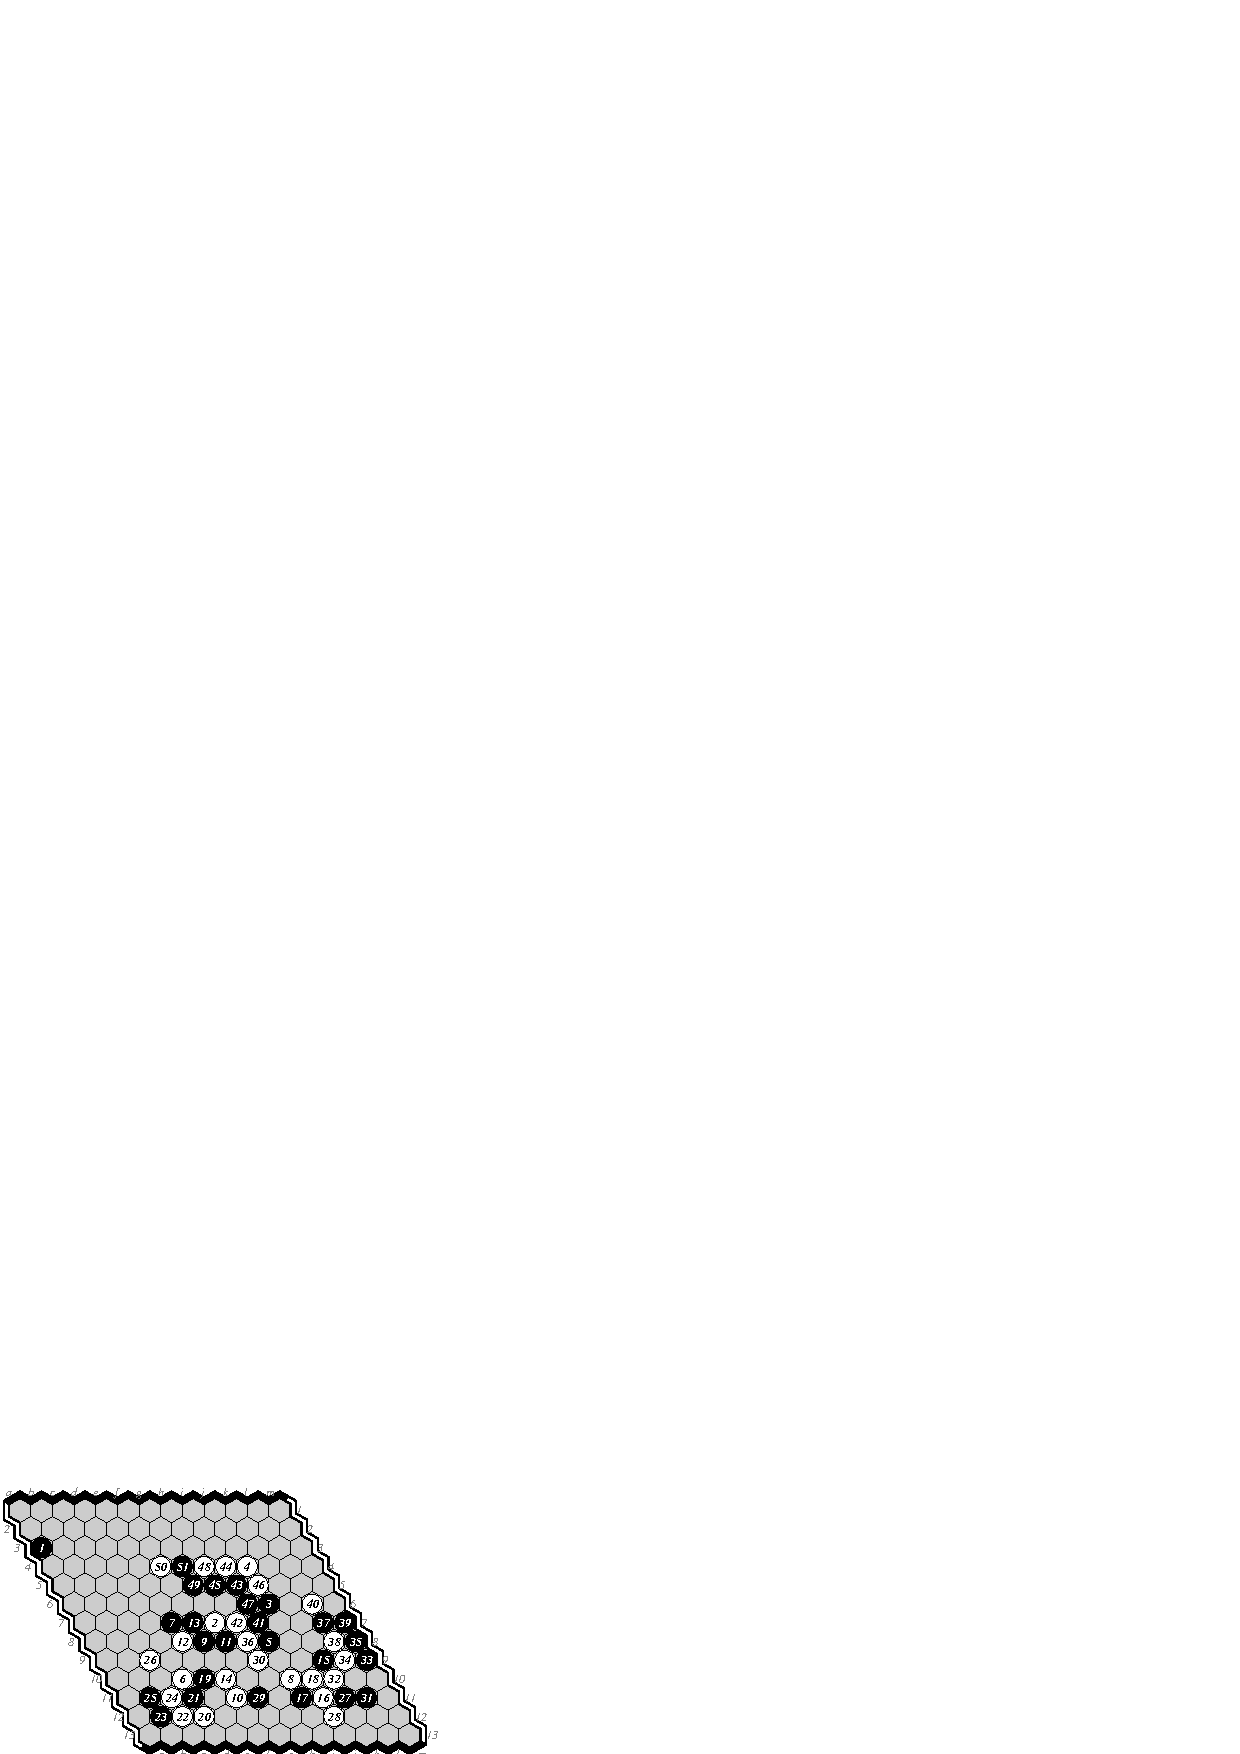
\includegraphics[width=.58\columnwidth]{pix/02-m-e}
\vspace*{.2cm}

\noindent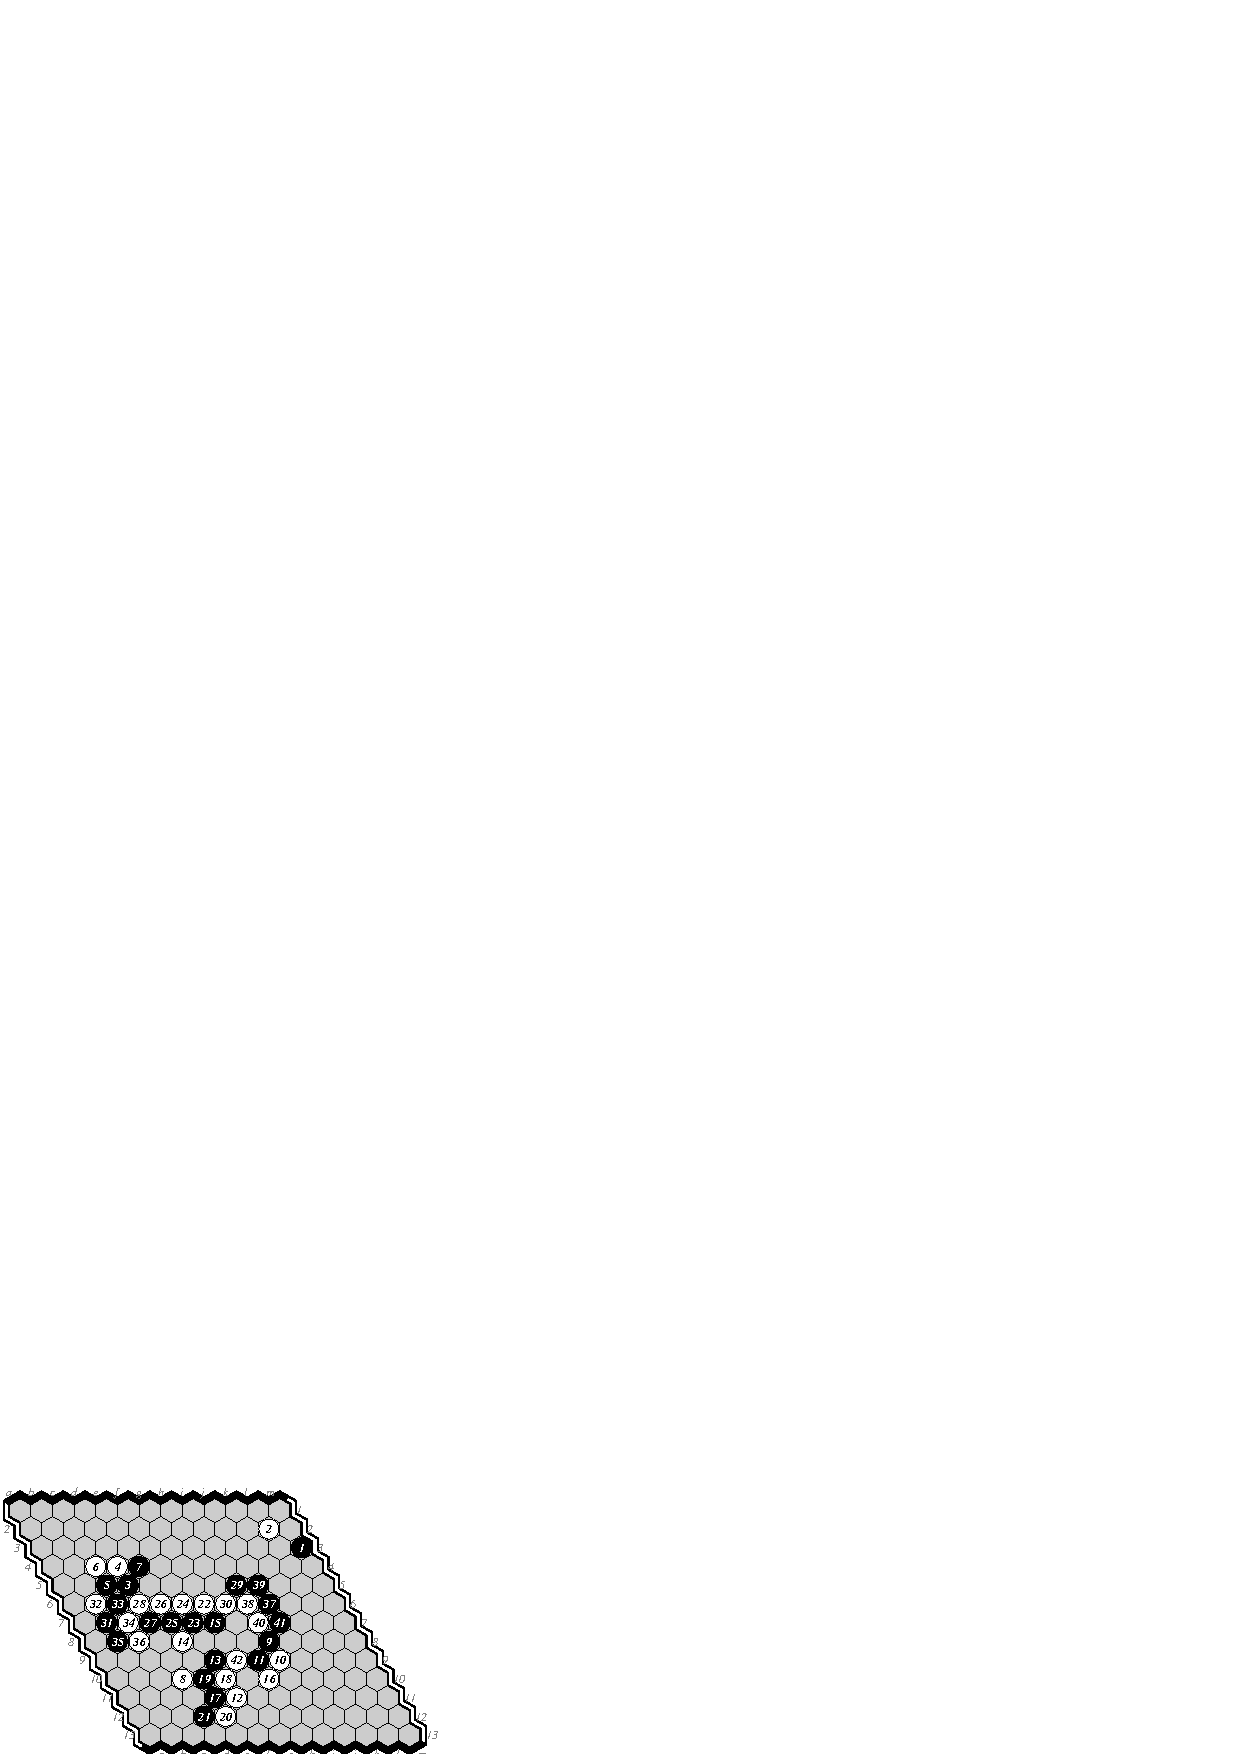
\includegraphics[width=.58\columnwidth]{pix/03-e-m}\hspace*{-.14\columnwidth}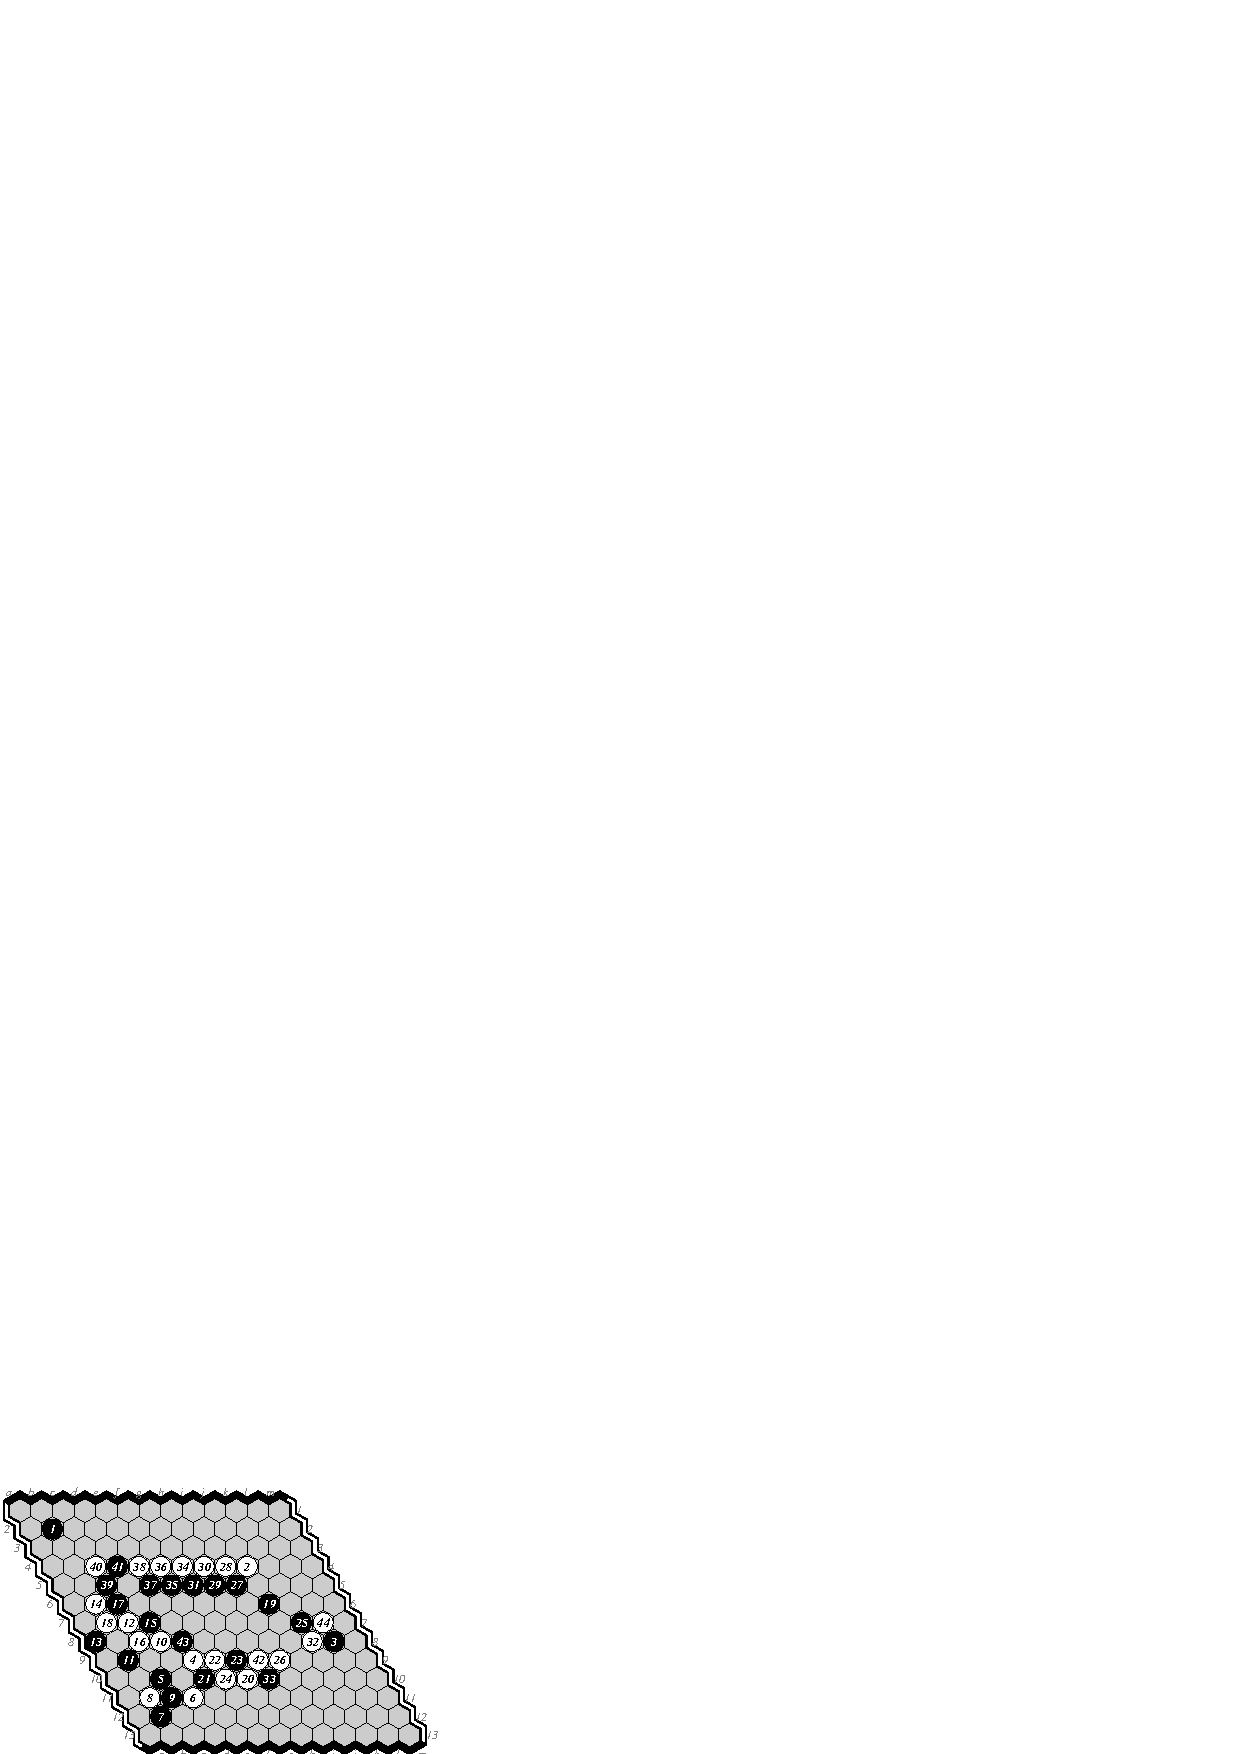
\includegraphics[width=.58\columnwidth]{pix/04-m-e}
\vspace*{.2cm}

\noindent\hfill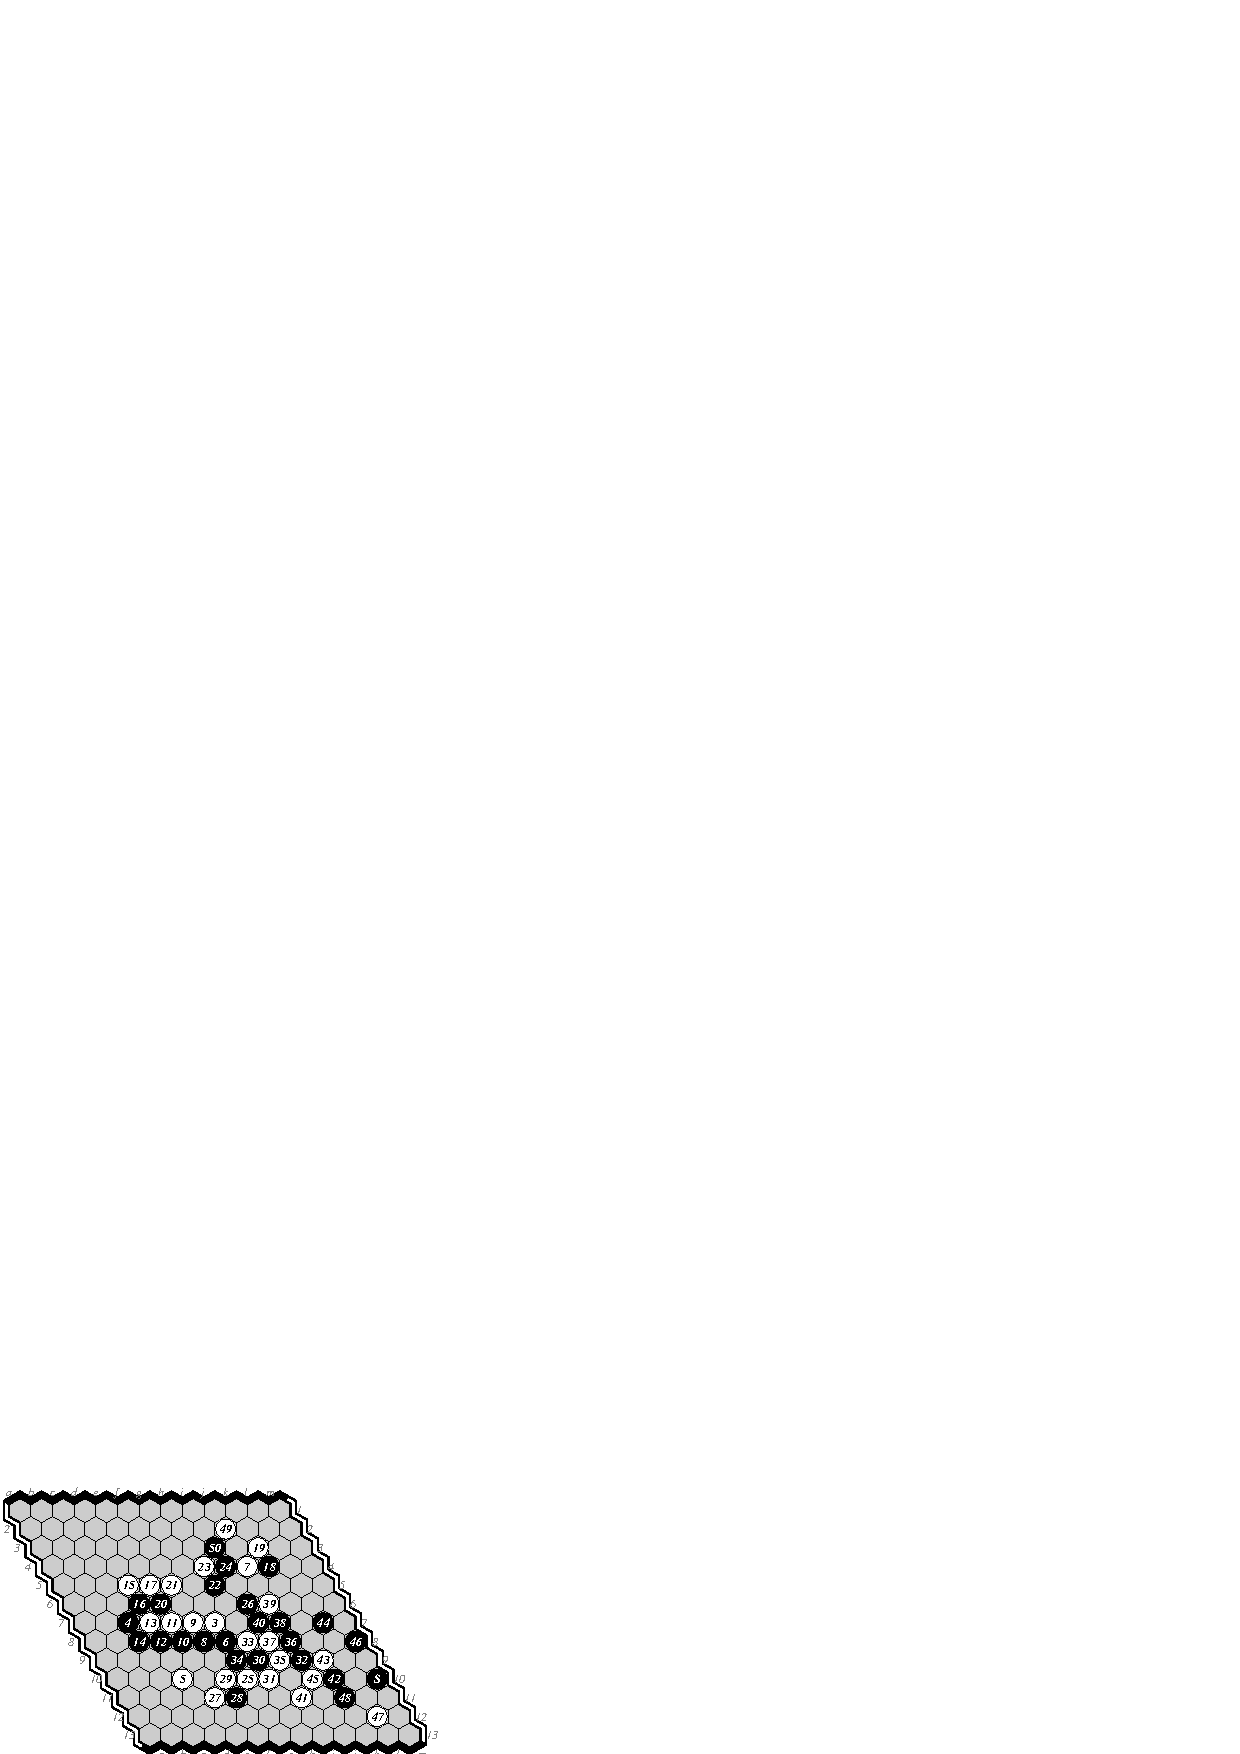
\includegraphics[width=.58\columnwidth]{pix/05-e-m}\hfill\ 
\caption{13$\times$13 Games 1-5. E-M 0-1, M-E 1-0, E-M 0-1, M-E 1-0, E-M 0-1.}
\end{figure}

\section{11$\times$11 Games.}
\begin{figure}
\noindent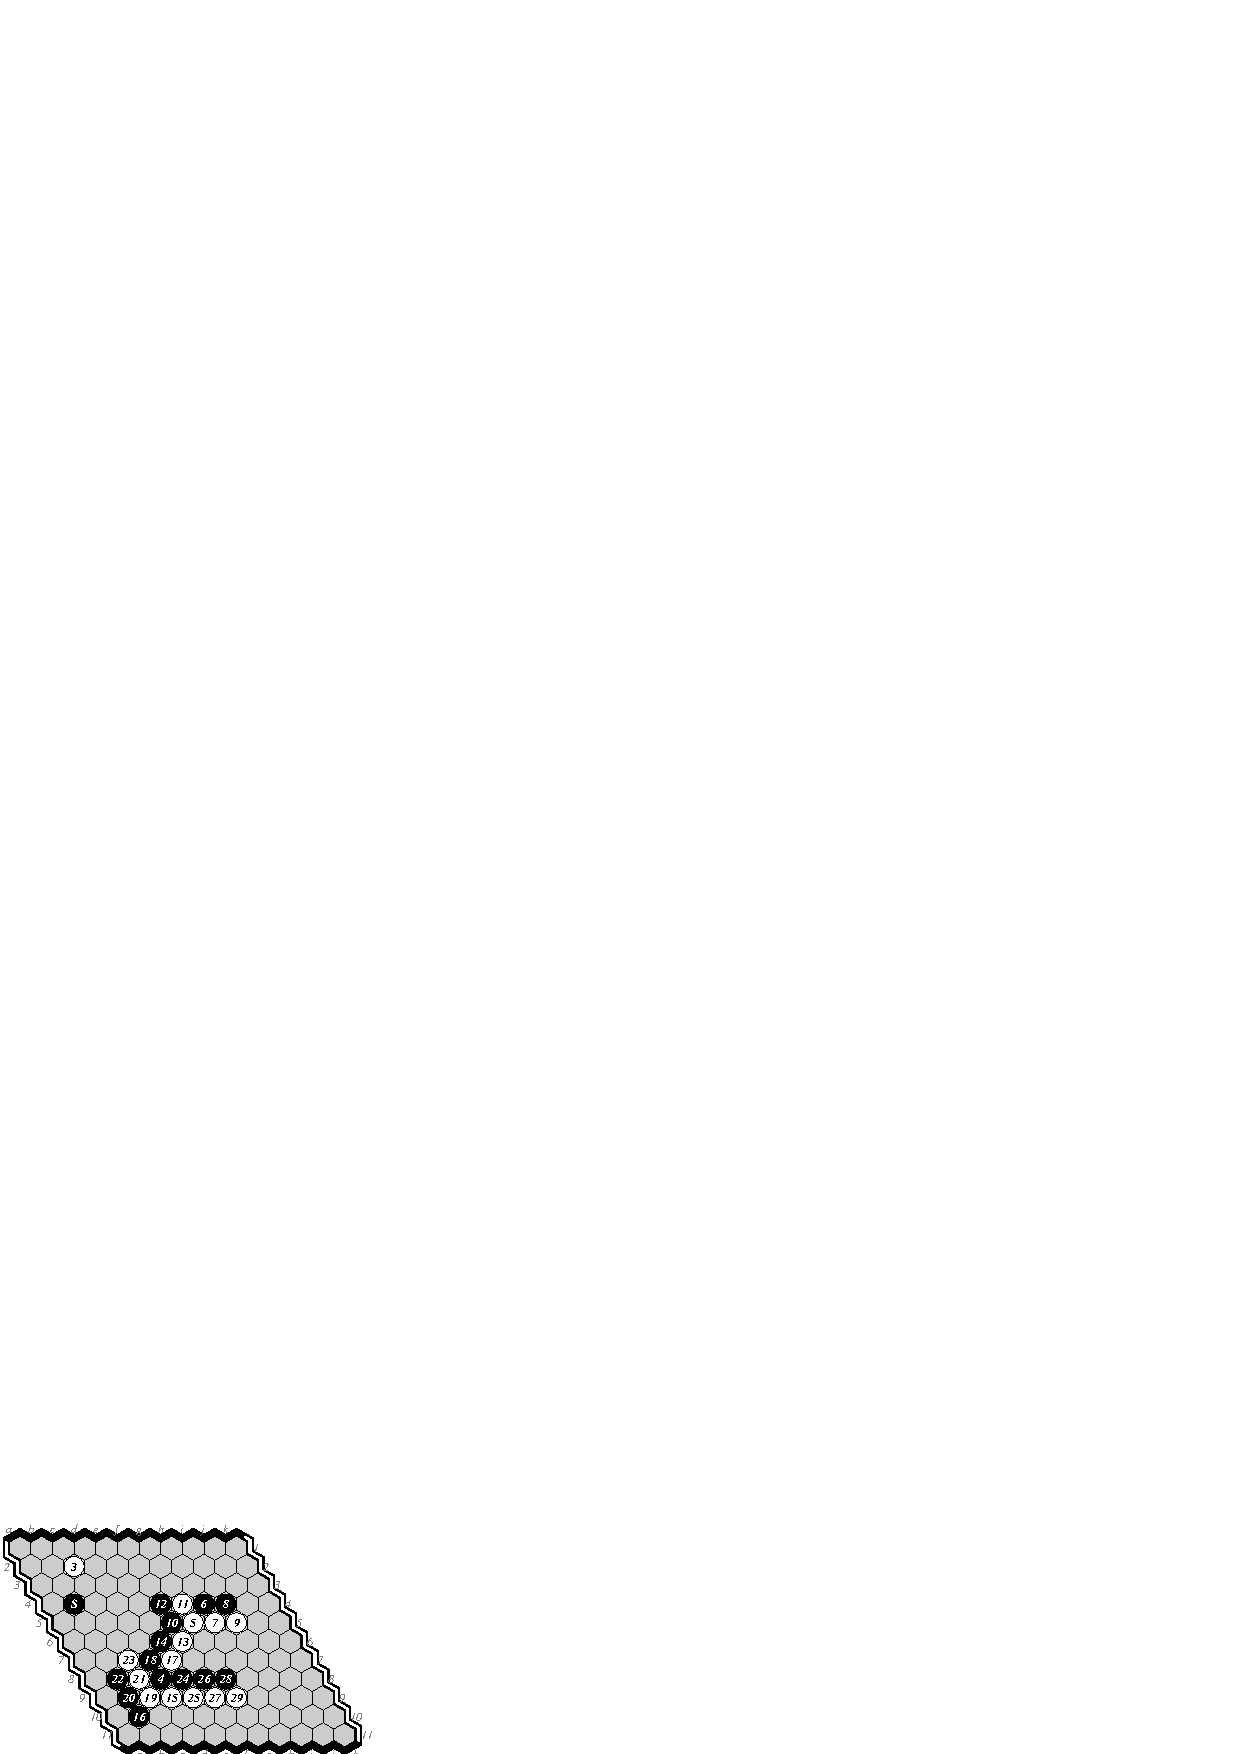
\includegraphics[width=.58\columnwidth]{pix/11-01-me}\hspace*{-.14\columnwidth}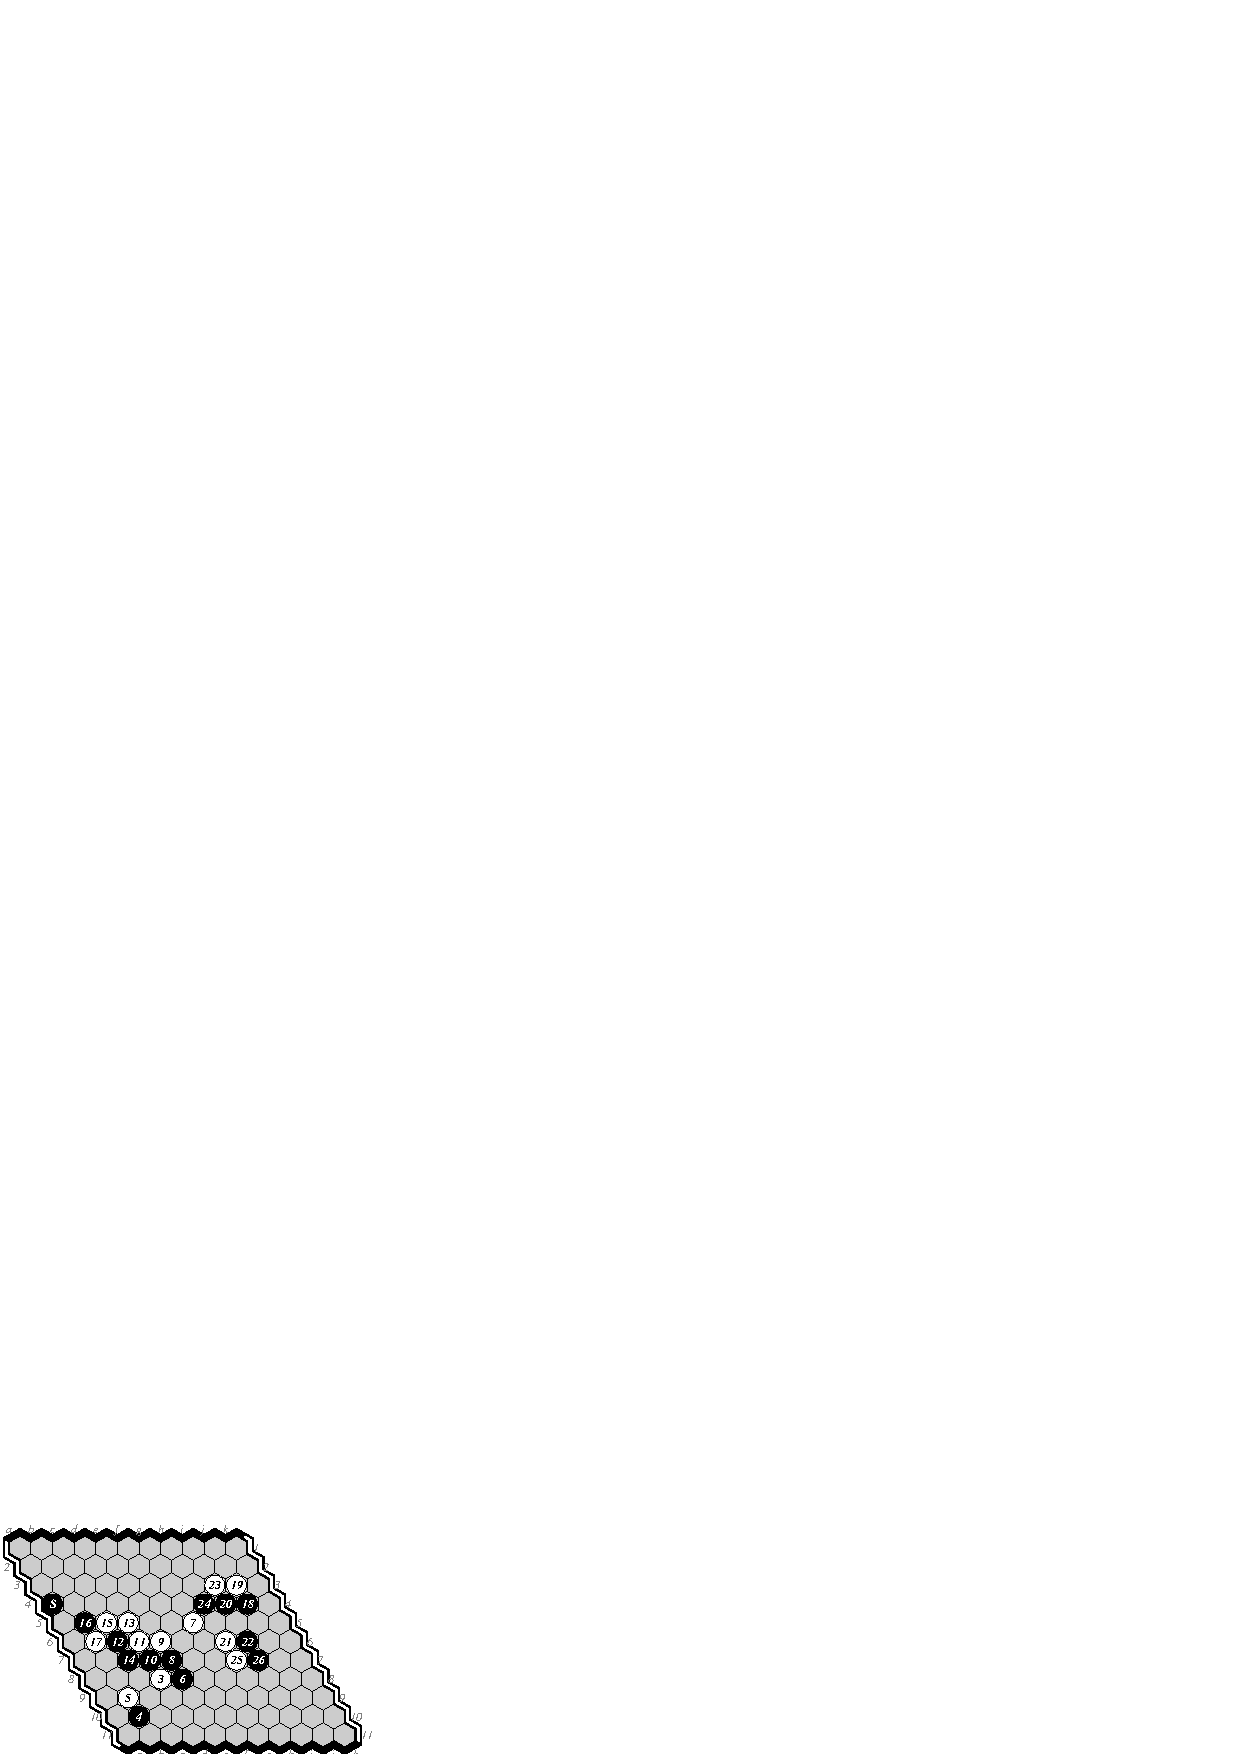
\includegraphics[width=.58\columnwidth]{pix/11-02-em}
\vspace*{.2cm}

\noindent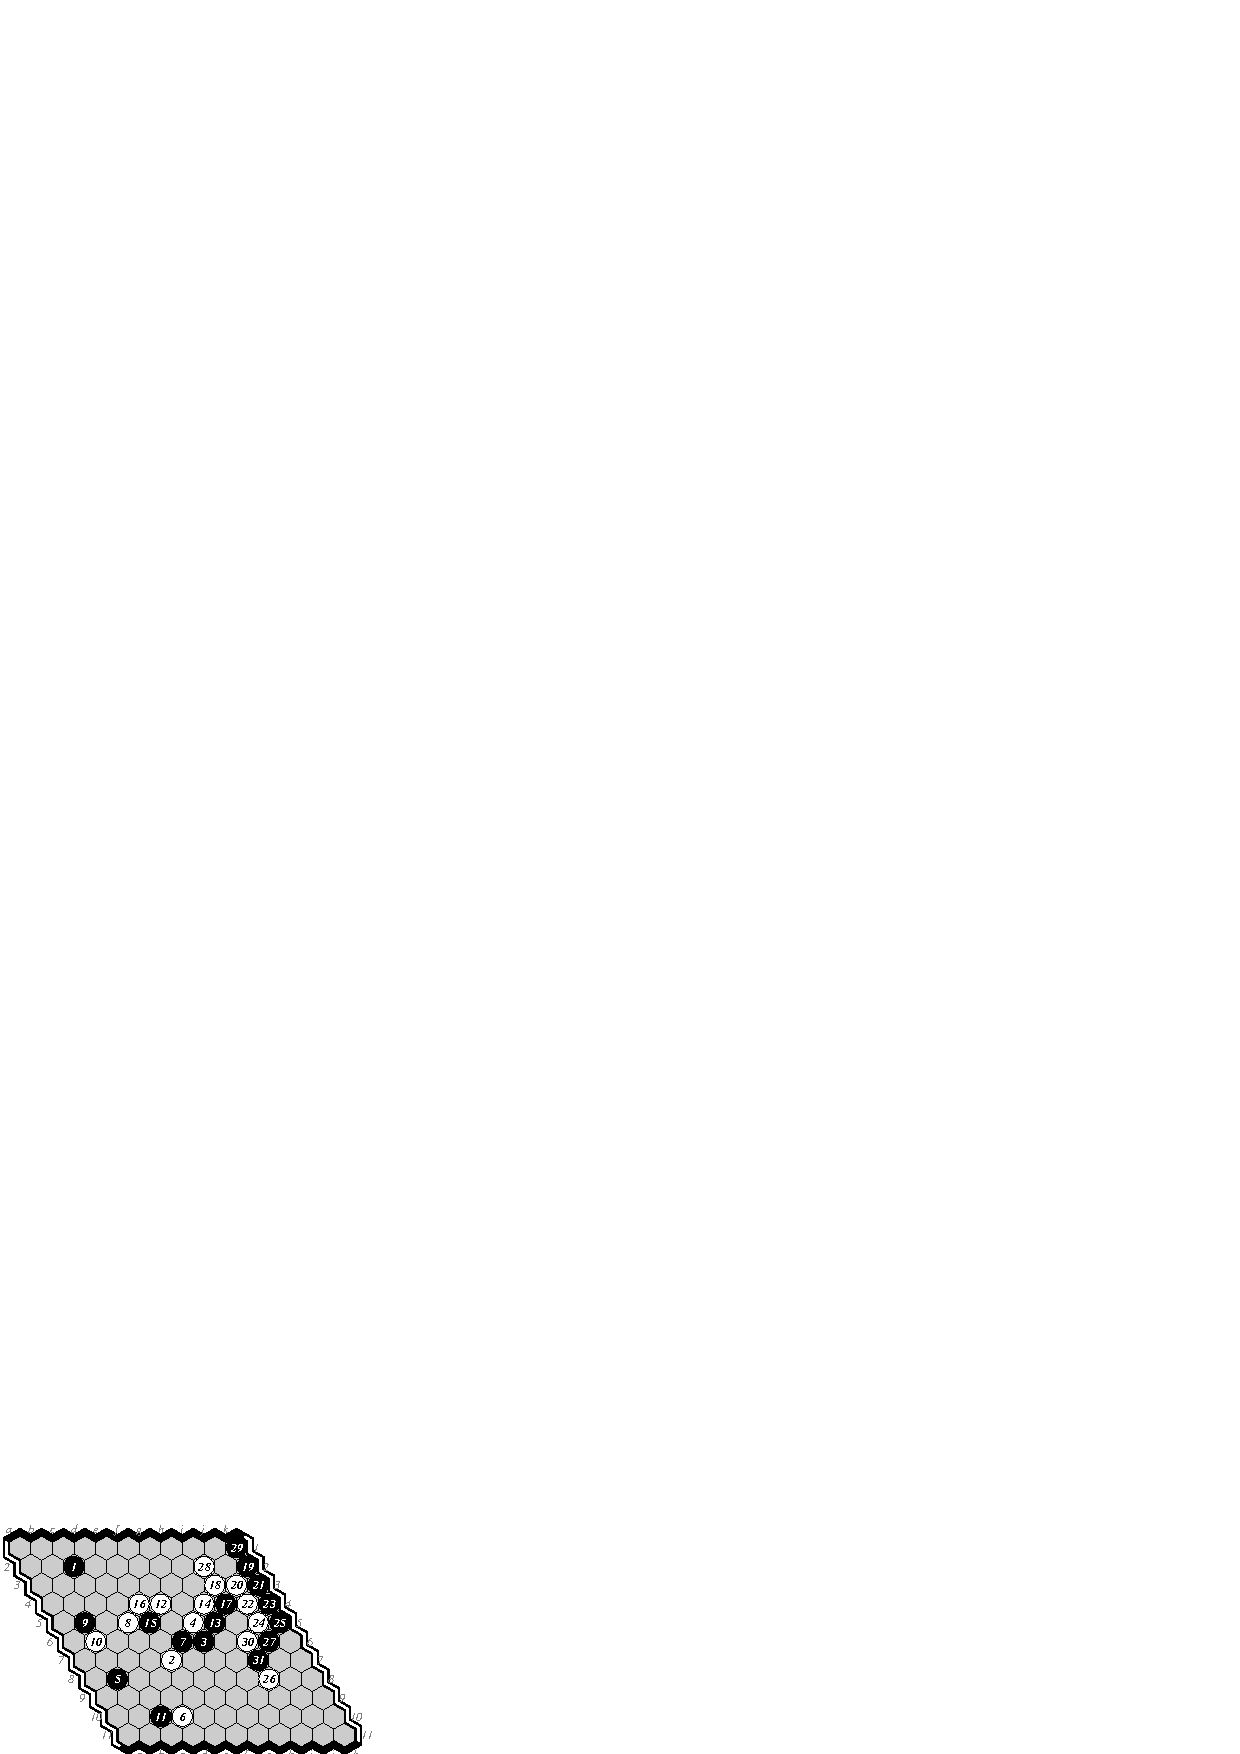
\includegraphics[width=.58\columnwidth]{pix/11-03-me}\hspace*{-.14\columnwidth}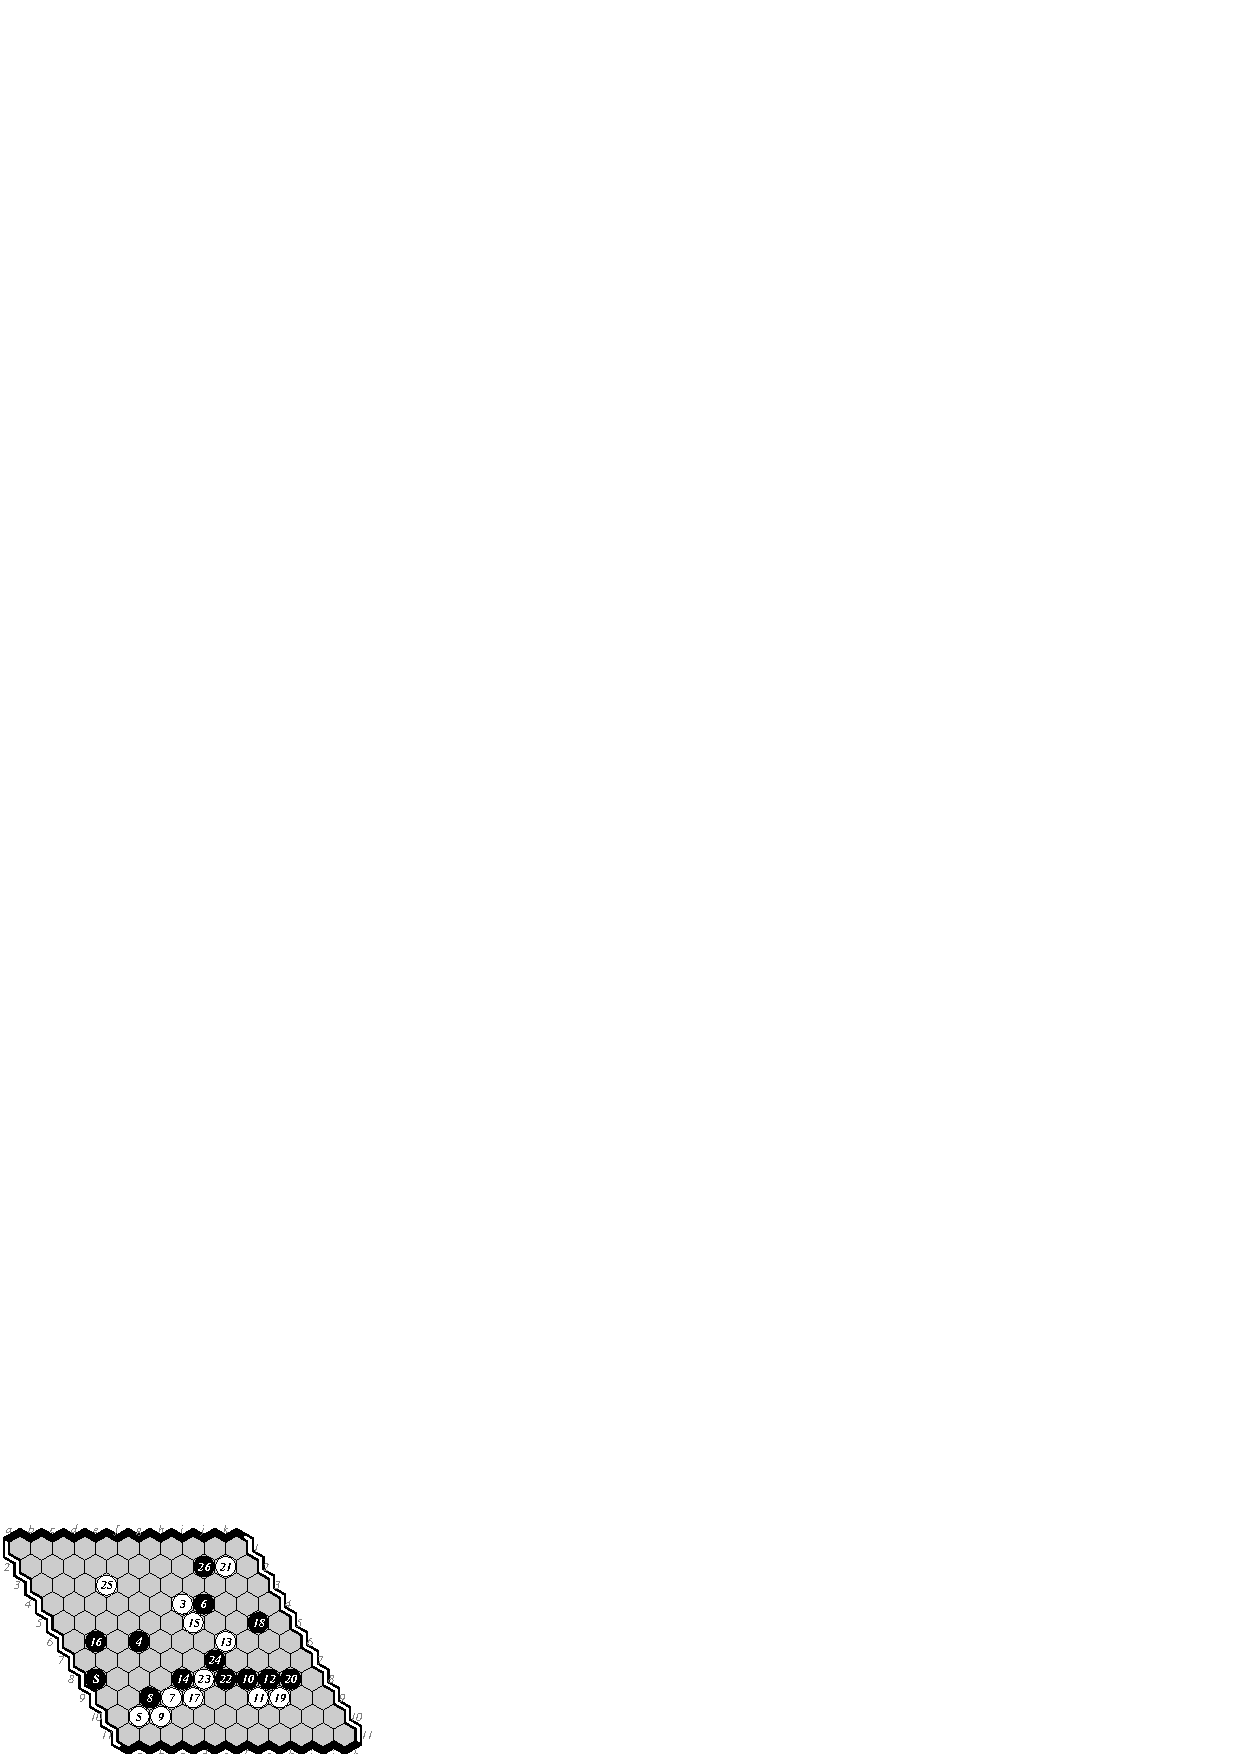
\includegraphics[width=.58\columnwidth]{pix/11-04-em}
\vspace*{.2cm}

\noindent\hfill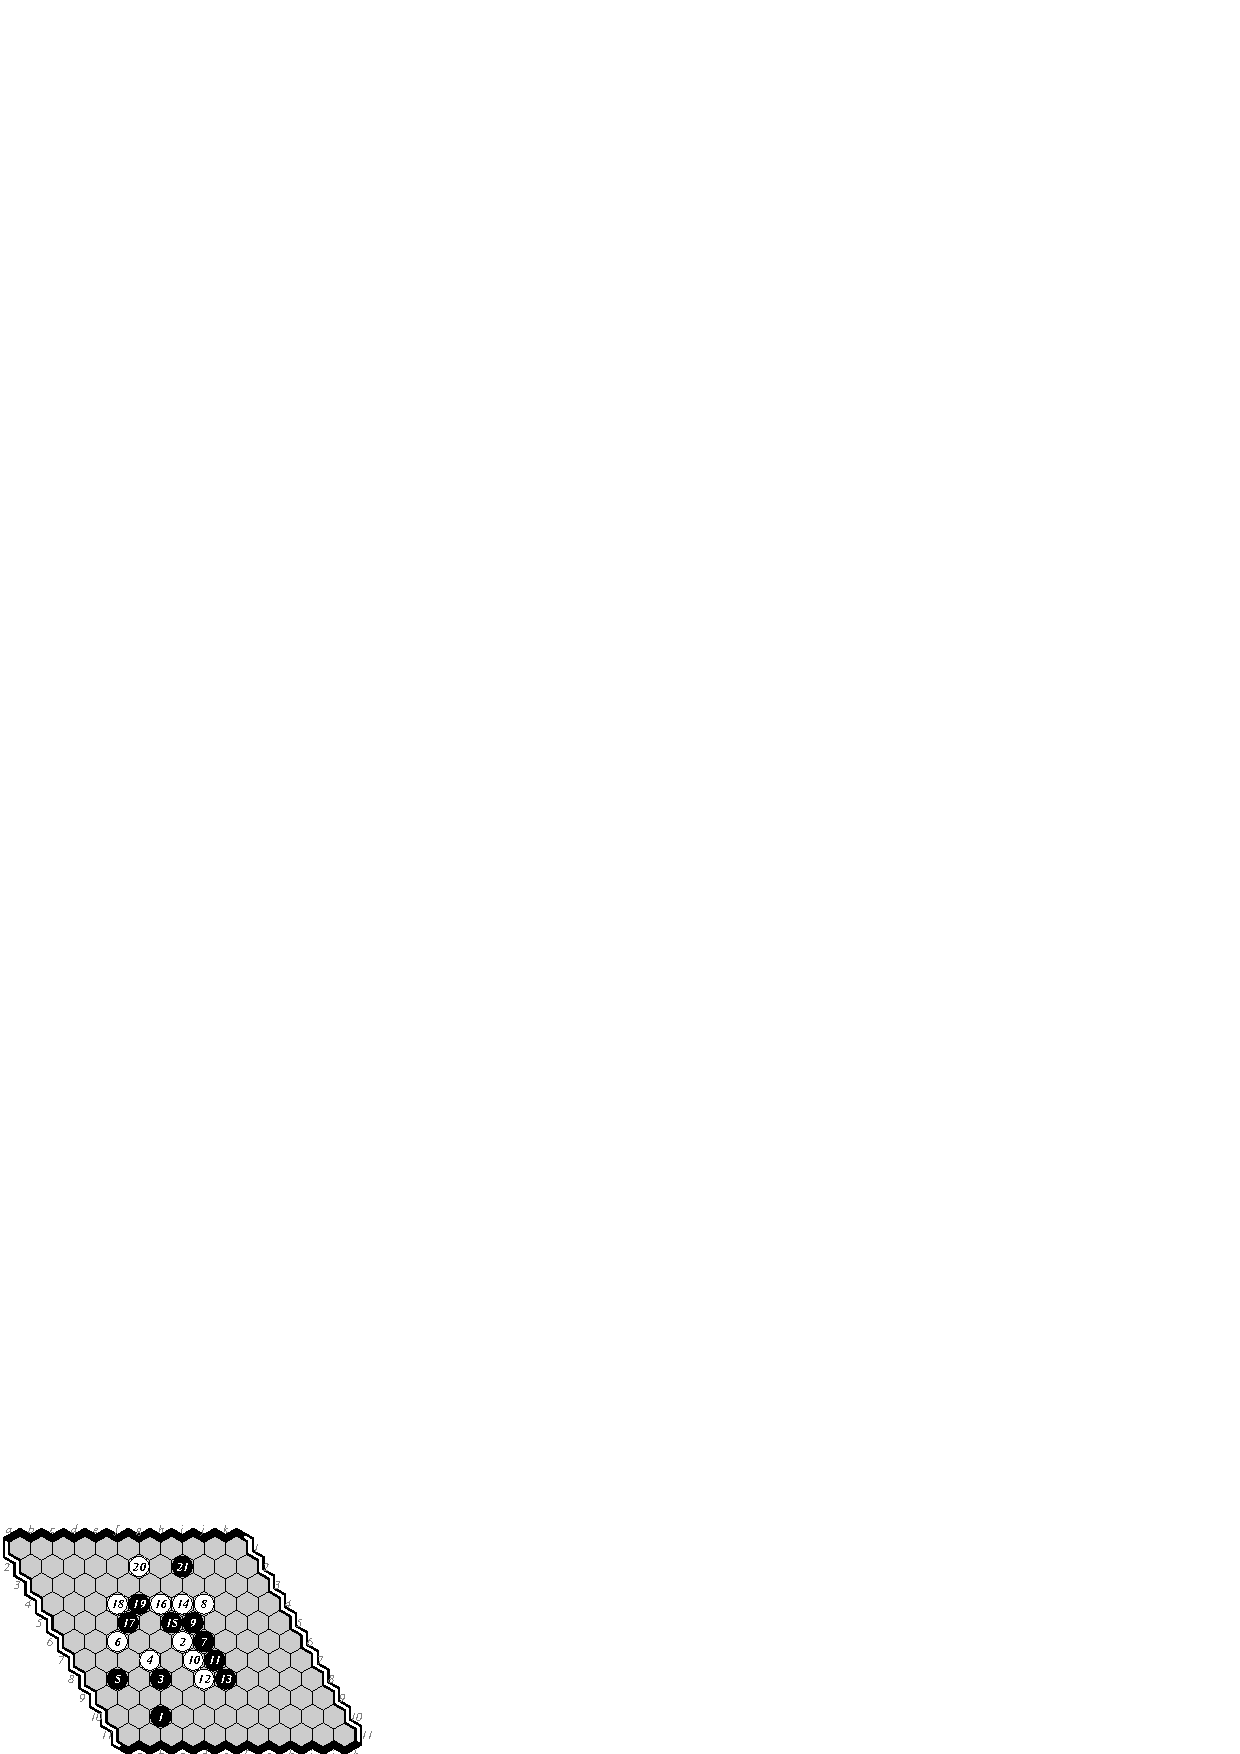
\includegraphics[width=.58\columnwidth]{pix/11-05-me}\hfill\ 
\caption{11$\times$11 Games 1-5. M-E 1-0, E-M 0-1, M-E 1-0, E-M 0-1, M-E 1-0.}
\end{figure}

\section{Conclusions}
TODO

\section*{Acknowledgements}
We thank the NSERC Discovery Grant Program for research funding.
\bibliographystyle{plain}
\bibliography{rpt}
\end{document}
